\documentclass[11pt,a4paper]{article}
\usepackage[utf8]{inputenc}
\usepackage[T1]{fontenc}
\usepackage{lmodern}
\usepackage{textcomp}
\usepackage{amsmath,amssymb}
\usepackage{graphicx}
\usepackage{booktabs}
\usepackage{longtable}
\usepackage{array}
\usepackage{listings}
\usepackage{xcolor}
\usepackage[margin=1in]{geometry}
\usepackage{float}
\usepackage[hidelinks,breaklinks]{hyperref}
\usepackage{microtype}
\setlength{\parskip}{4pt}
\lstset{basicstyle=\ttfamily\scriptsize,breaklines=true,breakatwhitespace=false,
  postbreak=\mbox{\textcolor{gray}{$\hookrightarrow$}\space},frame=single,
  framerule=0.3pt,rulecolor=\color{gray!60},columns=fullflexible,keepspaces=true,
  showstringspaces=false,numbers=none,xleftmargin=4pt,xrightmargin=4pt,
  literate={\_}{{\_}}1}
\graphicspath{{figures/}}
\providecommand{\tightlist}{}
\title{Lyman-$\alpha$ Warm Dark Matter Limits Compared with Non-Resonant Sterile-Neutrino Production}
\author{HEP-Genesis-Agent session record \\ \small Project: ramp-combo-lyman-wdm}
\date{2026-10-19}
\begin{document}
\maketitle
\noindent\textit{\small This document is an AI-generated account of an interactive session with the HEP-Genesis agent. Its text was written by a language model strictly from the session record; figures and numbers come only from tool results obtained during the session. The supplementary material and the transcript, generated alongside, document exactly what ran. Verify independently before use.}
\vspace{1em}

\begin{abstract}
We survey recent Lyman-$\alpha$ forest lower limits on the thermal-relic warm dark matter (WDM) mass and compare them with non-resonantly produced (Dodelson--Widrow, DW) keV sterile neutrinos. The relic-density and production-fraction calculations use a sterile-neutrino production server. The thermal-relic limits were read from paper text or abstracts. They span $m_x>3.1$~keV (Villasenor et al.\ 2022) to $m_x>5.7$~keV (Ir?i? et al.\ 2023) at 95\% CL. Thermal-history and $k_{\rm max}$ choices weaken them to 3.5--4.1~keV. Equation~5 of Viel et al.\ (2005), verified in the paper text, maps these limits to DW-equivalent masses of $\approx 20$--$45$~keV. An alternative Bozek-type relation, whose coefficients could not be traced to any paper, gives 17--37~keV. On the server, $\Omega_s h^2$ is linear in $\sin^2 2\theta$ and scales roughly as $m_s^{1.8}$. Its DW relic curve ($\Omega_s h^2=0.12$) runs from $\sin^2 2\theta = 2.5\times10^{-10}$ at 7.1~keV to $8.8\times10^{-12}$ at 46~keV. A hand comparison with the Abazajian (2005) fitting formula puts the literature relic mixing 10--16 times higher than the server's. The server's DW fractions would then be overstated by 1.5--2 orders of magnitude. This comparison was flagged as contested by the session's critic. The server's own X-ray limits exclude pure DW dark matter at 7.1 and 20~keV and have no coverage at 29--46~keV. The NuSTAR Galactic Center paper implies exclusion of the DW line above $\sim16$~keV, but only by inference from its wording, which is also contested. Pure DW production as all of the dark matter therefore appears excluded. The X-ray-allowed fraction $f_X(m_s)$ could not be tabulated because numerical NuSTAR mixing limits were not extracted.
\end{abstract}

\section{Introduction}

The user asked for three things. The first was a survey of recent Lyman-$\alpha$ forest constraints on warm dark matter. The second was a comparison of those constraints with sterile neutrinos produced non-resonantly (the Dodelson--Widrow mechanism). The third was to use the available sterile-neutrino tools to compute production fractions $f=\Omega_s/\Omega_{\rm DM}$.

Lyman-$\alpha$ analyses usually express their results as a lower limit on the mass $m_x$ of an early-decoupled thermal relic. Comparing these with DW sterile neutrinos needs three further ingredients:
\begin{enumerate}
\item a mapping from $m_x$ to the equivalent non-resonant sterile-neutrino mass $m_s$;
\item the DW relic-abundance curve in the $(m_s,\sin^2 2\theta)$ plane;
\item X-ray radiative-decay limits on the mixing angle at the resulting masses, together with mixed cold-plus-warm Lyman-$\alpha$ bounds if DW neutrinos form only a fraction of the dark matter.
\end{enumerate}

The session followed six lines of work in turn. These were the server-based DW production calculation, verification of the Lyman-$\alpha$ limits and of the mass conversion, the X-ray and mixed-model side, extraction of numerical NuSTAR limits (blocked), a cross-check of the server's DW yield against the literature, and a robustness test of the mass mapping with a search for post-2023 limits.

The automated pre-survey stated that no sterile-neutrino tools were available. This was wrong: the server was present and was used, and that statement is corrected here.

\section{Methods}

\paragraph{Sterile-neutrino server.} The production server (\texttt{serve-sbbn.sh}) maps $(m_s,\sin^2 2\theta,\text{mechanism})$ to several outputs: $\Delta N_{\rm eff}$, $\Omega_s h^2$, BBN abundances, radiative-decay quantities and a free-streaming length. Its BBN abundances ($Y_p$, D/H, $^7$Li/H) come from a fit to the PRyMordial network accurate to better than 0.3\%. BBN exclusion is defined as $\Delta\chi^2>3.84$ relative to the Standard Model.

The server's skill recipe gives the decay line at $E_\gamma=m_s/2$ with rate
\[
\Gamma = 1.36\times10^{-32}\,{\rm s^{-1}}\,\left(\frac{\sin^2 2\theta}{10^{-10}}\right)\left(\frac{m_s}{\rm keV}\right)^5 .
\]
X-ray fluxes are whole-halo values that assume the sterile neutrino is all of the dark matter, with no field-of-view cut. Exclusion verdicts compare against an internal table of limits "within 30\% in mass"; the limit values themselves are not returned.

\paragraph{Server runs.} All runs used the DW mechanism with local execution:
\begin{itemize}
\item a single point at $m_s=7.1$~keV, $\sin^2 2\theta=5\times10^{-11}$;
\item a five-mass grid at $\sin^2 2\theta=10^{-9}$;
\item a $15\times13$ grid over $m_s=1$--50~keV and $\sin^2 2\theta=10^{-13}$--$10^{-7}$;
\item a $5\times2$ grid at 22--50~keV with $\sin^2 2\theta = 10^{-12}$ and $10^{-11}$;
\item a five-point "zip" run on the derived relic curve;
\item X-ray line predictions at the relic-curve points;
\item an $80\times80$ scan over $m_s=1$--100~keV and $\sin^2 2\theta=10^{-14}$--$10^{-6}$, together with its exclusion plot.
\end{itemize}

\paragraph{Literature.} Papers were found with arXiv abstract search and metadata queries. Full text was downloaded and read in chunks for the following papers:
\begin{itemize}
\item Viel et al.\ 2005 (arXiv:astro-ph/0501562);
\item Ir?i? et al.\ 2023 (arXiv:2309.04533);
\item Ir?i? et al.\ 2017 (arXiv:1702.01764);
\item Perez et al.\ 2017 (arXiv:1609.00667);
\item Abazajian 2005 (arXiv:astro-ph/0511630).
\end{itemize}
The other papers were used at abstract level only.

An attempt to extract Figs.~6--8 of arXiv:1609.00667 failed: the HTML and ar5iv renderings contained only Figs.~3 and 4. Several derived numbers were computed by hand by the assistant and not by any tool. These include the mass conversions, the literature relic mixings, the revised fractions, the NuSTAR flux estimate and the $\Delta N_{\rm eff}$ estimate, and they are flagged as hand calculations throughout. A critic reviewed each stage. The full tool-call log is in the supplement.

\section{Results}

\subsection{Lyman-$\alpha$ thermal-relic limits}

Table~\ref{tab:lya} collects the limits that were verified. Full text was read for arXiv:1702.01764 and arXiv:2309.04533. The limits from arXiv:1306.2314, arXiv:1911.09073 and arXiv:2209.14220 were taken from abstracts.

The spread among the recent limits, 3.1 to 5.7~keV, is comparable to the shifts caused by modelling choices: 5.3$\to$3.5~keV from the thermal history and 5.7$\to$4.1~keV from $k_{\rm max}$. Small-scale modelling, including the IGM thermal history, peculiar-velocity smearing and inhomogeneous reionization, is therefore the dominant uncertainty.

For historical context, the abstract of Viel et al.\ 2005 (arXiv:astro-ph/0501562) quotes $m_{\rm WDM}\gtrsim550$~eV ($2\sigma$) for thermal relics.

\begin{table}
\centering
\begin{tabular}{llll}
\toprule
Analysis & Data & $m_x$ limit & Systematic variation \\
\midrule
Viel+2013 (1306.2314) & HIRES/MIKE, $z>4$ & $>3.3$ keV ($2\sigma$) & 1, 2, 2.5 keV disfavoured at $\sim$9, 4, 3$\sigma$ \\
Ir?i?+2017 (1702.01764) & XQ-100 / HIRES/MIKE / joint & 1.4 / 4.1 / 5.3 keV ($2\sigma$) & joint $\to$3.5 keV with $T$ jumps $\le5000$ K \\
Palanque-Delabrouille+2019 (1911.09073) & SDSS DR14 $z<4.5$ + XQ-100 & $>5.3$ keV (95\%) & -- \\
Villasenor+2022 (2209.14220) & 1080 Cholla runs, $z=4.0$--5.2 & $>3.1$ keV (95\%) & likelihood peak at 4.5 keV \\
Ir?i?+2023 (2309.04533) & HIRES/UVES, $z=4.2$--5.0 & $>5.7$ keV (95\%) & 4.1 keV for $k_{\rm max}<0.1$ s/km \\
\bottomrule
\end{tabular}
\caption{Thermal-relic WDM limits verified in the session. In Villasenor+2022 the flux-power suppression saturates at $k\gtrsim0.1$ s/km because of peculiar-velocity smearing. Ir?i?+2023 uses $k_{\rm max}=0.2$ s/km for its headline limit.}
\label{tab:lya}
\end{table}

Three searches for post-2023 limits returned nothing relevant. One targeted a DESI thermal-relic limit, and two targeted P1D, eBOSS and emulator re-analyses. The results were DESI BAO and sample papers (arXiv:2404.03001, arXiv:2503.14739) or unrelated papers. The Rogers \& Peiris emulator framework (arXiv:2007.13751) was found, but its abstract quotes no WDM limit.

\subsection{Mapping thermal-relic to DW masses}

\paragraph{The Viel+2005 relation.} The paper text of arXiv:astro-ph/0501562 gives (Eq.~5)
\[
m_s^{\rm DW}=4.43\,{\rm keV}\,(m_x/{\rm keV})^{4/3}\,(0.25\cdot0.7^2/\omega_x)^{1/3},
\]
normalised at $\omega_x=0.1225$. The paper states that the correspondence is one-to-one when the transfer functions are identical.

The pre-survey had quoted a 4.46~keV prefactor from memory. That value does not appear in the paper. It equals the paper's value rescaled to $\omega_{\rm dm}=0.12$, since $4.43\times(0.1225/0.12)^{1/3}=4.461$~keV.

\paragraph{Converted masses.} Table~\ref{tab:map} gives the hand-computed DW-equivalent masses. The Bozek-type column, $3.9\,{\rm keV}\,m_x^{1.294}$, is unverified: its coefficients came from the planning notes and could not be confirmed in any paper text. The critic marked this two-relation comparison as contested. Under the alternative relation the DW-equivalent range moves down by 3.1--8.0~keV, from 20--45~keV to 17--37~keV.

\begin{table}
\centering
\begin{tabular}{cccc}
\toprule
$m_x$ (keV) & Viel+2005, $\omega=0.1225$ & Viel+2005, $\omega=0.12$ & Bozek-type (unverified) \\
\midrule
3.1 & 20.0 & 20.2 & 16.9 \\
3.3 & 21.8 & 21.9 & 18.3 \\
3.5 & 23.5 & 23.7 & 19.7 \\
4.1 & 29.1 & 29.3 & 24.2 \\
4.5 & 32.9 & 33.1 & -- \\
5.3 & 40.9 & 41.2 & 33.8 \\
5.7 & 45.1 & 45.4 & 37.1 \\
\bottomrule
\end{tabular}
\caption{DW/NRP-equivalent masses in keV, computed by hand by the assistant.}
\label{tab:map}
\end{table}

\paragraph{Directly quoted NRP masses.} Of the abstracts checked, only Boyarsky et al.\ (arXiv:0812.0010) quote non-resonant-production masses directly: $m_{\rm NRP}>8$~keV (frequentist 99.7\%) and $>12.1$~keV (Bayesian 95\%). Inverting Viel+2005 by hand, these correspond to $m_x\approx1.56$ and 2.12~keV, which is weaker than the modern limits. The DW masses for the other analyses therefore rest entirely on a mapping relation. It was not checked whether arXiv:2209.14220 or arXiv:1306.2314 quote NRP masses of their own.

\subsection{DW production on the server}

\paragraph{Scaling and relic curve.} On the server, $\Omega_s h^2$ is exactly linear in $\sin^2 2\theta$ and scales roughly as $m_s^{1.8}$. For example, at $\sin^2 2\theta=10^{-9}$ the server gives $\Omega_s h^2 = 0.4715$, 3.041, 5.936 and 11.07 at 7.1, 20, 29 and 41~keV.

Solving for $\Omega_s h^2=0.12$ gives the server's relic curve:
\begin{itemize}
\item $8.7\times10^{-9}$ (1 keV), $2.5\times10^{-9}$ (2 keV), $1.2\times10^{-9}$ (3 keV), $4.8\times10^{-10}$ (5 keV);
\item $2.5\times10^{-10}$ (7.1 keV), $1.4\times10^{-10}$ (10 keV), $6.6\times10^{-11}$ (15 keV);
\item $3.9\times10^{-11}$ (20 keV), $3.3\times10^{-11}$ (22 keV), $2.0\times10^{-11}$ (29 keV);
\item $1.08\times10^{-11}$ (41 keV), $8.8\times10^{-12}$ (46 keV), $7.6\times10^{-12}$ (50 keV).
\end{itemize}

A direct run on this curve confirmed $\Omega_s h^2=0.12$ at all five test points: $\sin^2 2\theta=2.545\times10^{-10}$, $3.946\times10^{-11}$, $2.022\times10^{-11}$, $1.084\times10^{-11}$ and $8.81\times10^{-12}$ at 7.1, 20, 29, 41 and 46~keV. The corresponding radiative lifetimes are $1.6\times10^{27}$, $5.82\times10^{25}$, $1.77\times10^{25}$, $5.85\times10^{24}$ and $4.05\times10^{24}$~s. The tool nonetheless flagged three of these points as "overcloses". The assistant attributed this to a threshold or rounding quirk.

\paragraph{Fractions at fixed mixing.} The server's fractions $f=\Omega_s h^2/0.12$ were marked contested by the critic. They are:
\begin{itemize}
\item at 7.1~keV and $\sin^2 2\theta=5\times10^{-11}$: $f=0.196$ ($\Omega_s h^2=0.0236$, ``19.6\% of $\Omega_{\rm DM}$'');
\item at $\sin^2 2\theta=10^{-12}$: $f=0.025$, 0.030, 0.049, 0.092 and 0.114 at 20, 22, 29, 41 and 46~keV;
\item at $10^{-11}$: ten times these values, with 46 and 50~keV overclosing ($\Omega_s h^2=0.136$, 0.158).
\end{itemize}

\paragraph{Other outputs.} The free-streaming length is 151~kpc at 7.1~keV, 107~kpc at 10~keV and 53.7~kpc at 20~keV. The server provides no momentum distribution, $\langle p/T\rangle$ or transfer function, so the free-streaming comparison of the DW and thermal-relic spectra could not be done with this tool.

At the 7.1~keV, $5\times10^{-11}$ point, the server gives the following BBN-related outputs:
\begin{itemize}
\item $\Delta N_{\rm eff}=3.09\times10^{-4}$;
\item $Y_p=0.24682$ and ${\rm D/H}\times10^5=2.4434$;
\item $\Delta\chi^2_{\rm BBN}=-0.004$, i.e.\ allowed.
\end{itemize}

The BBN-allowed maximum mixing from the scan falls from $3.93\times10^{-7}$ at 1~keV to $1.5\times10^{-8}$ near 50~keV and $9.43\times10^{-9}$ at 100~keV. This is far above the relic curve, so BBN does not constrain keV DW dark matter.

\paragraph{The exclusion plane.} The $80\times80$ scan contained 6400 points, of which 3092 overclose and 968 are BBN-excluded. Figure~\ref{fig:10} shows the resulting exclusion plane. It overlays the overclosure region, the $\Omega_{\rm DM}$ line, NuSTAR/XMM limits, a Lyman-$\alpha$ thermal-WDM bound and the 3.5~keV point.


\begin{figure}[H]
\centering
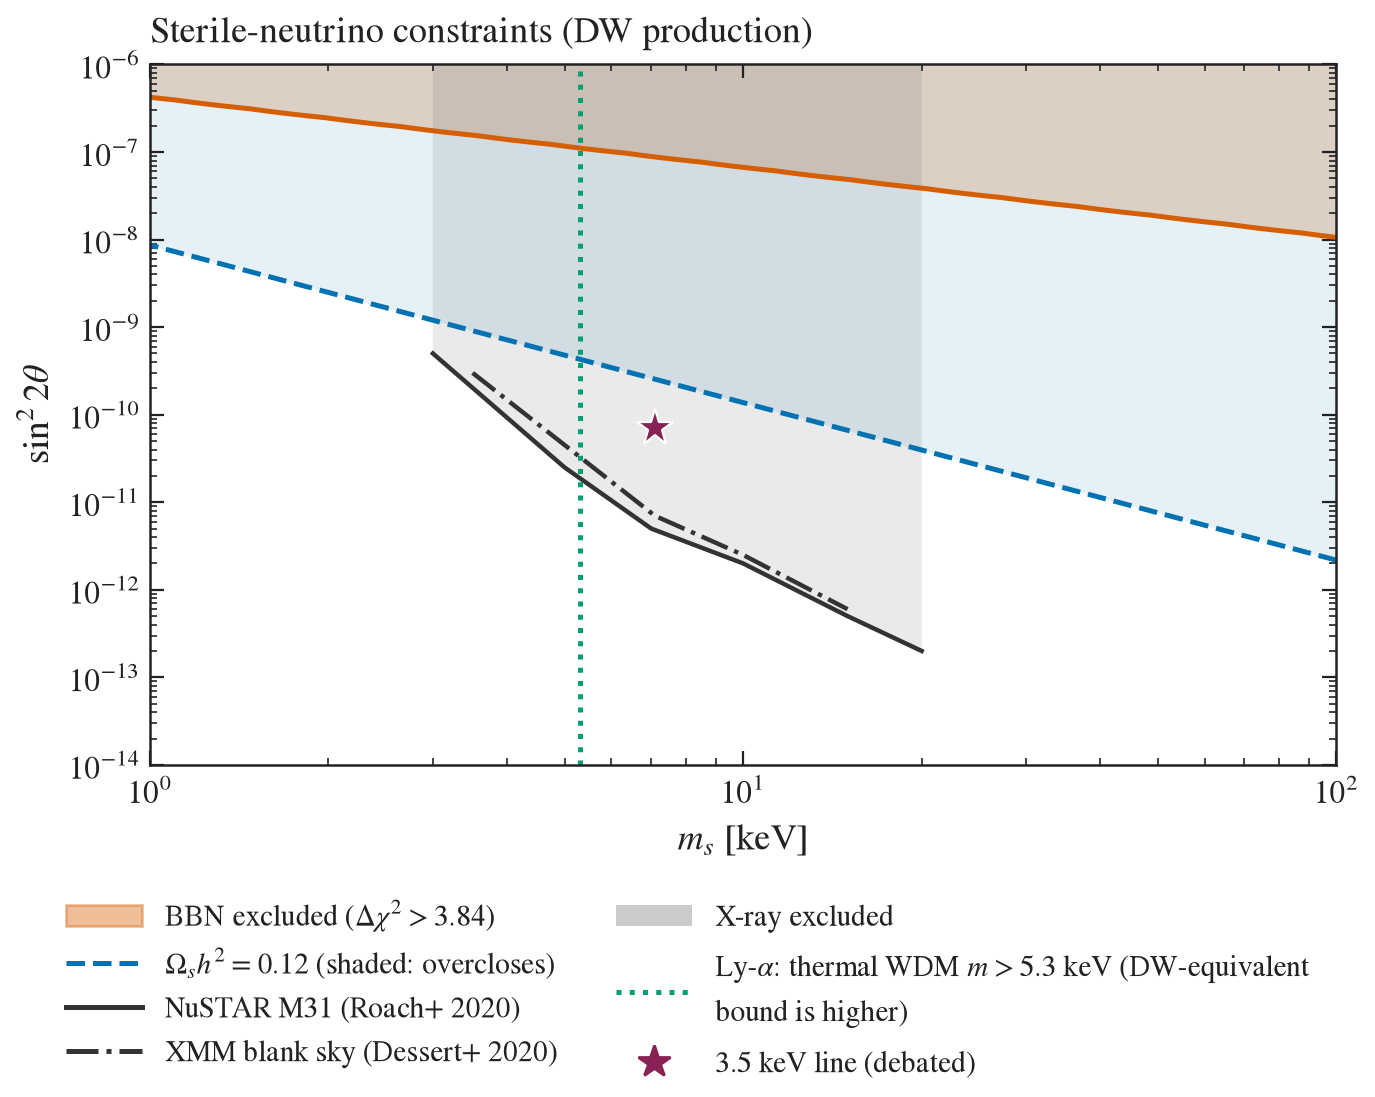
\includegraphics[width=0.85\textwidth,height=0.6\textheight,keepaspectratio]{fig-10.png}
\caption{exclusion\_scan\_DW\_d94a06.png Produced in this session by \texttt{plot\_sterile\_nu\_exclusion} on \textit{serve-sbbn.sh}.}
\label{fig:10}
\end{figure}



The plot summarises the server's view of the DW parameter space. Three caveats limit its use as a constraint figure:
\begin{itemize}
\item the tool does not document where its overlaid X-ray and Lyman-$\alpha$ curves come from;
\item its internal X-ray table has no coverage at 29--46~keV, so the absence of an X-ray boundary there is a gap rather than an allowed region;
\item its relic line uses the server normalisation, which the cross-check below finds 10--16 times too low in mixing.
\end{itemize}

\subsection{X-ray decay and the mixed cold-plus-warm bound}

\paragraph{Predicted lines at the relic points.} At the server's relic mixings, the line energies are $E_\gamma=3.55$, 10, 14.5, 20.5 and 23~keV for $m_s=7.1$, 20, 29, 41 and 46~keV.

The whole-halo M31 fluxes are $1.75\times10^{-3}$, $1.71\times10^{-2}$, $3.88\times10^{-2}$, $8.31\times10^{-2}$ and 0.107~ph\,s$^{-1}$\,cm$^{-2}$. The corresponding Milky Way centre fluxes are 11.9, 116, 264, 564 and 727~ph\,s$^{-1}$\,cm$^{-2}$.

\paragraph{The server's verdicts.} The tool reports the following:
\begin{itemize}
\item at 7.1~keV: excluded by NuSTAR M31 (Roach+2020) and XMM-Newton blank sky (Dessert+2020);
\item at 20~keV: excluded by NuSTAR M31;
\item at 29, 41 and 46~keV: "Not excluded by tabulated X-ray limits (within 30\% in mass)".
\end{itemize}
The last verdict means there is no coverage, not that these masses are allowed. The tool never returns the limit value itself. The finding built on these verdicts was contested by the critic, and a later check confirmed that the "not excluded" result at 29~keV reflects missing coverage.

\paragraph{NuSTAR Galactic Center limits.} Perez et al.\ (arXiv:1609.00667) describe their NuSTAR Galactic Center limits as the strongest over most of 10--50~keV. The text states that, within the $\nu$MSM, their limit implies $m_\chi\lesssim16$~keV. It also states that the $\nu$MSM band in their Fig.~8 is bounded above by the non-resonant production line, and that INTEGRAL rules out mixing-produced sterile neutrinos as all of the dark matter above 50~keV.

The assistant inferred from this wording that pure DW is X-ray-excluded at 20, 29, 41 and 46~keV. A weakening ("bump") of the limit near 40~keV makes 41~keV the least secure point. This inference is contested and has medium confidence.

\paragraph{Predicted NuSTAR aperture flux.} Equation~5 of arXiv:1609.00667 gives
\[
F\approx2.6\times10^{-6}\,{\rm cm^{-2}s^{-1}}\,\left(\frac{m}{20\,{\rm keV}}\right)^4\left(\frac{\sin^2 2\theta}{10^{-14}}\right)\left(\frac{d\Omega}{4\,{\rm deg^2}}\right)\left(\frac{J}{40\,{\rm GeV\,cm^{-3}\,kpc\,sr^{-1}}}\right),
\]
with $d\Omega_{\rm tot}\approx3.8$~deg$^2$ and $J_{\rm tot}=29$~GeV\,cm$^{-3}$\,kpc\,sr$^{-1}$ for the coreNFW profile. Applied by hand to the server's 20~keV relic mixing, it predicts $\approx7\times10^{-3}$~ph\,cm$^{-2}$\,s$^{-1}$ in the 0-bounce aperture. This estimate is contested. The numerical limits for comparison appear only in Figs.~6--8 of that paper, which could not be extracted.

\paragraph{Mixed cold-plus-warm bound.} Boyarsky et al.\ (arXiv:0812.0010) allow any $m_{\rm NRP}$ in $5\,{\rm keV}<m_{\rm NRP}<\infty$ when $F_{\rm WDM}<0.6$ (frequentist 99.7\%) or $F_{\rm WDM}<0.35$ (Bayesian 95\%). The planned comparison of an X-ray-allowed fraction $f_X(m_s)$ with this bound was blocked, because no numerical NuSTAR $\sin^2 2\theta$ limits at 20--46~keV were obtained.

\subsection{Cross-check of the server's DW yield}

\paragraph{The literature fit.} Abazajian 2005 (arXiv:astro-ph/0511630, Eq.~7, read in the text) gives
\[
m_s=3.40\,{\rm keV}\left(\frac{\sin^2 2\theta}{10^{-8}}\right)^{-0.615}\left(\frac{\Omega_{\rm DM}}{0.26}\right)^{0.5}\times\left\{0.527\,{\rm erfc}\!\left[-1.15\left(\frac{T_{\rm QCD}}{170\,{\rm MeV}}\right)^{2.15}\right]\right\},
\]
valid for $135<T_{\rm QCD}<300$~MeV. The braced factor equals 1 at $T_{\rm QCD} = 170$~MeV. Inverting gives $\Omega_s\propto(\sin^2 2\theta)^{1.23}m_s^2$, whereas the server is linear in mixing and scales roughly as $m_s^{1.8}$. The paper also gives the peak production temperature as $T_{\rm peak}\approx130\,{\rm MeV}\,(m_s/3\,{\rm keV})^{1/3}$.

\paragraph{Comparison of relic mixings.} The hand-computed literature relic mixings are compared with the server's in Table~\ref{tab:xcheck}. The ratios are 10--16 and grow with mass. The critic's earlier estimate of a factor of 2.5 understated the gap. All findings in this cross-check were marked contested, and the planned \texttt{cite} entry for Eq.~7 was not made.

\begin{table}
\centering
\begin{tabular}{cccc}
\toprule
$m_s$ (keV) & Literature $\sin^2 2\theta$ & Server $\sin^2 2\theta$ & Ratio \\
\midrule
3 & $1.23\times10^{-8}$ & $1.2\times10^{-9}$ & 10.2 \\
7.1 & $3.02\times10^{-9}$ & $2.5\times10^{-10}$ & 12.1 \\
20 & $5.61\times10^{-10}$ & $3.9\times10^{-11}$ & 14.4 \\
29 & $3.06\times10^{-10}$ & $2.0\times10^{-11}$ & 15.3 \\
41 & $1.75\times10^{-10}$ & $1.08\times10^{-11}$ & 16.1 \\
46 & $1.45\times10^{-10}$ & $8.8\times10^{-12}$ & 16.4 \\
\bottomrule
\end{tabular}
\caption{DW relic mixing from the Abazajian 2005 fit, computed by hand with $\Omega_{\rm DM}=0.26$ and $T_{\rm QCD}=170$~MeV, compared with the server's relic curve.}
\label{tab:xcheck}
\end{table}

\paragraph{Revised fractions.} Rescaling with $f=(\sin^2 2\theta/\sin^2 2\theta_{\rm relic})^{1.23}$ gives the fractions below. These are hand calculations and are contested.
\begin{itemize}
\item At 7.1~keV: $f=0.0064$ for $\sin^2 2\theta = 5\times10^{-11}$ and 0.0098 for $7\times10^{-11}$, compared with the server's 0.196 and 0.27. The assistant described this as consistent with the literature statement of $\sim1\%$ of the dark matter at the 3.5~keV-line mixing.
\item At $\sin^2 2\theta=10^{-12}$: $f=4.2\times10^{-4}$ (20 keV), $8.8\times10^{-4}$ (29 keV), $1.75\times10^{-3}$ (41 keV) and $2.2\times10^{-3}$ (46 keV). These are 50--60 times below the server's values.
\item At $10^{-11}$: no point overcloses.
\end{itemize}

\paragraph{$\Delta N_{\rm eff}$ on the relic curve.} On the relic curve the sterile number density is fixed by $\Omega_s h^2/m_s$, whichever yield normalisation is used. A hand estimate assuming one Weyl species gives $\Delta N_{\rm eff}\approx 11.3\,{\rm eV}/m_s$: $1.6\times10^{-3}$ at 7.1~keV, $5.6\times10^{-4}$ at 20~keV and $2.5\times10^{-4}$ at 46~keV.

This agrees with the server's own on-curve value of $1.574\times10^{-3}$ at 7.1~keV. It corrects the earlier statement that $\Delta N_{\rm eff}$ is at most $3\times10^{-4}$, which holds only above $\sim40$~keV. All values are 2--3 orders of magnitude below BBN and Planck sensitivity, so BBN does not constrain keV DW dark matter.

\section{Discussion}

The question was how Lyman-$\alpha$ WDM limits compare with non-resonant sterile-neutrino production. The Lyman-$\alpha$ side is the most secure part of the session. The thermal-relic limits are 3.1--5.7~keV, and under Viel+2005 they correspond to $m_s^{\rm DW}\gtrsim20$--45~keV. The conversion assumes that the DW spectrum is a rescaled Fermi--Dirac distribution. An unverified alternative relation lowers the DW-equivalent range to 17--37~keV, and the session could not determine which relation is more appropriate.

The X-ray side is less firm. The server's verdicts exclude pure DW at 7.1 and 20~keV but give no limit values and have no coverage above about 26~keV. The exclusion at 29--46~keV rests on the assistant's reading of the Perez et al.\ text, which the critic contested. The "bump" in the NuSTAR limit near 40~keV may weaken the case at 41~keV.

Taken together, a Lyman-$\alpha$ lower mass bound near 17--20~keV and an X-ray exclusion of the DW line above $\sim16$~keV leave no window for pure DW dark matter. This conclusion is qualitative. It is also consistent with the abstract of Asaka, Laine \& Shaposhnikov (arXiv:hep-ph/0612182), which states that DW as the sole dark matter is possible only below 3.5~keV (6~keV with relaxed assumptions). The abstract of arXiv:1512.05369 likewise states that DW cannot meet relic and structure-formation bounds simultaneously.

The largest methodological issue is the server's DW yield normalisation. If the hand comparison with Abazajian 2005 holds, the server overproduces DW sterile neutrinos at fixed mixing by a factor of order 10--16 in mixing. Its relic curve in Figure~\ref{fig:10} would then lie too low, and its fractions at fixed mixing would be too large by 1.5--2 orders of magnitude.

This correction strengthens rather than weakens the exclusion of pure DW, because a higher relic mixing is easier for X-ray limits to exclude. It does, however, make any server-based fraction $f$ unreliable without rescaling. The comparison itself has open dependencies: a single 2005 fit was used, and the later DW yields mentioned in the session (arXiv:1705.01837, Venumadhav et al.\ 2016) were not checked. The correction should be treated as provisional.

Several attempts failed or were blocked. Three literature searches for post-2023 DESI P1D or emulator WDM limits returned nothing relevant; the assistant judged the search tool's keyword ranking to be poor. Figure extraction from arXiv:1609.00667 failed because the HTML renderings lacked Figs.~6--8. The server's CSV could not be loaded with the table loader because of a header-parsing error and was read as text instead.

Finally, the server reports no $\langle p/T\rangle$, transfer function or half-mode wavenumber. The free-streaming comparison between the DW and thermal-relic spectra therefore remained unanswered.

\section{Conclusions}

Recent Lyman-$\alpha$ analyses bound the thermal-relic WDM mass at $m_x>3.1$--5.7~keV (95\% CL). Thermal-history and $k_{\rm max}$ choices loosen these to 3.5--4.1~keV. Viel+2005 Eq.~5, verified in the paper text, maps them to $m_s^{\rm DW}\approx20$--45~keV.

The sterile-neutrino server produced a DW relic curve and production fractions. A hand cross-check against Abazajian 2005 indicates that the server's relic mixings are 10--16 times too low and its fractions 50--60 times too high at fixed mixing. This result is contested.

Pure DW sterile neutrinos as all of the dark matter appear excluded by the combination of the Lyman-$\alpha$ lower mass bound with X-ray limits. Above $\sim20$~keV this rests on an inference from the NuSTAR paper's text rather than on numerical limits. The X-ray-allowed fraction $f_X(m_s)$ and its comparison with the Boyarsky+2009 mixed-model bound ($F_{\rm WDM}<0.35$--0.6) were not obtained.

The session left the following questions open:
\begin{enumerate}
\item Obtain numerical NuSTAR upper limits on $\sin^2 2\theta$ at 20, 29, 41 and 46~keV, from Perez+2017 Fig.~8, Roach+2020 (arXiv:1908.09037) or Roach+2023. Then tabulate $f_X$ and test it against the mixed-model bound.
\item Check whether updated DW yields (arXiv:1705.01837, Venumadhav+2016) shift the relic mixing from the 2005 fit and should be quoted as a range.
\item Search for post-2023 DESI P1D or emulator WDM limits using web search or author names.
\item Determine whether arXiv:2209.14220, arXiv:1911.09073 or arXiv:1306.2314 quote their own NRP-equivalent masses, and confirm the source of the Bozek-type relation.
\end{enumerate}

\section*{References}
\begin{itemize}
\item arXiv:astro-ph/0501562 --- M. Viel, J. Lesgourgues, M. G. Haehnelt, S. Matarrese, A. Riotto, Constraining Warm Dark Matter candidates including sterile neutrinos and light gravitinos with WMAP and the Lyman-alpha forest (2005).
\item arXiv:1306.2314 --- M. Viel, G. D. Becker, J. S. Bolton, M. G. Haehnelt, Warm Dark Matter as a solution to the small scale crisis: new constraints from high redshift Lyman-alpha forest data (2013).
\item arXiv:1702.01764 --- V. Ir?i?, M. Viel, M. G. Haehnelt, J. S. Bolton et al., New Constraints on the free-streaming of warm dark matter from intermediate and small scale Lyman-$\alpha$ forest data (2017).
\item arXiv:1911.09073 --- N. Palanque-Delabrouille, C. Yèche, N. Schöneberg, J. Lesgourgues et al., Hints, neutrino bounds and WDM constraints from SDSS DR14 Lyman-$\alpha$ and Planck full-survey data (2019).
\item arXiv:2209.14220 --- B. Villasenor, B. Robertson, P. Madau, E. Schneider, New Constraints on Warm Dark Matter from the Lyman-$\alpha$ Forest Power Spectrum (2022).
\item arXiv:2309.04533 --- V. Ir?i?, M. Viel, M. G. Haehnelt, J. S. Bolton et al., Unveiling Dark Matter free-streaming at the smallest scales with high redshift Lyman-alpha forest (2023).
\item arXiv:0812.0010 --- A. Boyarsky, J. Lesgourgues, O. Ruchayskiy, M. Viel, Lyman-alpha constraints on warm and on warm-plus-cold dark matter models (2008).
\item arXiv:1609.00667 --- K. Perez, K. C. Y. Ng, J. F. Beacom, C. Hersh, S. Horiuchi, R. Krivonos, (Almost) Closing the $\nu$MSM Sterile Neutrino Dark Matter Window with NuSTAR (2016).
\item arXiv:astro-ph/0511630 --- K. Abazajian, Production and Evolution of Perturbations of Sterile Neutrino Dark Matter (2005).
\item arXiv:hep-ph/0612182 --- T. Asaka, M. Laine, M. Shaposhnikov, Lightest sterile neutrino abundance within the nuMSM (2006).
\item arXiv:2007.13751 --- K. K. Rogers, H. V. Peiris, General framework for cosmological dark matter bounds using $N$-body simulations (2020).
\item arXiv:1705.01837 --- K. N. Abazajian, Sterile neutrinos in cosmology (2017).
\item arXiv:1512.05369 --- Dodelson-Widrow Production of Sterile Neutrino Dark Matter with Non-Trivial Initial Abundance.
\item arXiv:1908.09037 --- Roach et al.\ 2020 (NuSTAR M31; cited by identifier only).
\item arXiv:2404.03001 --- DESI 2024 IV: Baryon Acoustic Oscillations from the Lyman Alpha Forest.
\item arXiv:2503.14739 --- DESI DR2 Results I: Baryon Acoustic Oscillations from the Lyman Alpha Forest.
\end{itemize}

\section*{Data and code availability}
All outputs of this session are collected in the project folder \href{file:///Users/nramachandra/hep-genesis-testing/projects/ramp-combo-lyman-wdm}{\texttt{/\allowbreak{}Users/\allowbreak{}nramachandra/\allowbreak{}hep-genesis-testing/\allowbreak{}projects/\allowbreak{}ramp-combo-lyman-wdm}}.
The session produced 12 data files; the supplement lists them.
Full documentation of how these results were obtained is in the supplementary material (\texttt{supplement.pdf}: implementation details, the tool-call log, the research board with every finding and its evidence, figures not shown here, and the code index) and the verbatim transcript (\texttt{transcript.pdf}), generated alongside this report.


\end{document}
